% ------------------------------------------------------------------------------
% TYPO3 Version 10.4 - What's New (Serbian Version)
%
% @license	Creative Commons BY-NC-SA 3.0
% @link		https://typo3.org/help/documentation/whats-new/
% @language	Serbian
% ------------------------------------------------------------------------------

\section{Izmene za integratore}
\begin{frame}[fragile]
	\frametitle{Izmene za integratore}

	\begin{center}\huge{Poglavlje 2:}\end{center}
	\begin{center}\huge{\color{typo3darkgrey}\textbf{Izmene za integratore}}\end{center}

\end{frame}

% ------------------------------------------------------------------------------
% Feature | 89513 | Provide password recovery for backend users

\begin{frame}[fragile]
	\frametitle{Izmene za integratore}
	\framesubtitle{Mejl za povratak izgubljene lozinke (1)}

	\begin{itemize}

		\item Zahtev za povratak izgubljene lozinke za korisnike administratorskog interfejsa je validan samo 4 sata.\newline
			Vremensko ograničenje se ne može menjati.
		\item Zbog dodatne sigurnosti ova funkcionalnost može da se onemogući za administratore ili za sve korisnike.
		\item Ukoliko više korisnika koristi istu mejl adresu, koristi se alternativni tekst.
		\item TCA polje \texttt{be\_users.email} se ne sme postaviti na opciju \texttt{eval=email}.

		\item Ova funkcionalnost radi samo za korisnike koji:
			\begin{itemize}
				\item imaju unešenu mejl adresu,
				\item postavljenu lozinku
				\item i nisu onemogućeni/izbrisani.
			\end{itemize}

	\end{itemize}

\end{frame}

% ------------------------------------------------------------------------------
% Feature | 89513 | Provide password recovery for backend users

\begin{frame}[fragile]
	\frametitle{Izmene za integratore}
	\framesubtitle{Mejl za povratak izgubljene lozinke (2)}

	\begin{itemize}
		\item Mejl za povratak izgubljene lozinke se takodje može poslati putem komandne linije.
	\end{itemize}

	\begin{figure}
		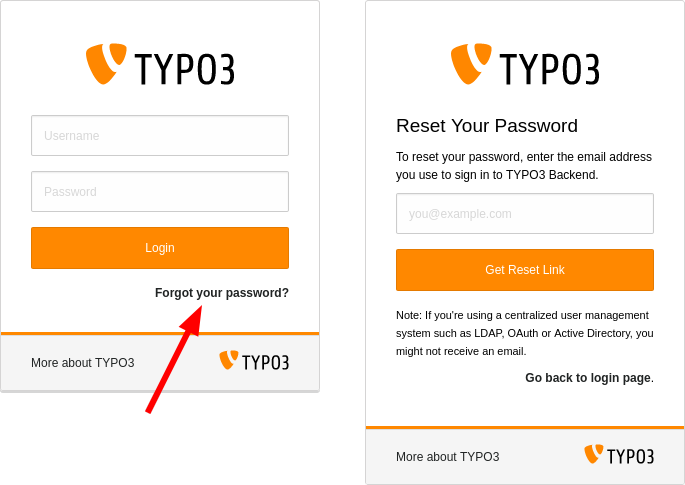
\includegraphics[width=0.9\linewidth]{ChangesForIntegrators/89513-ProvidePasswordRecoveryForBackendUsers.png}
	\end{figure}

\end{frame}

% ------------------------------------------------------------------------------
% Important | 90285 | Fresh installs without constraint for typo3fluid/fluid will get version 3.0+

\begin{frame}[fragile]
	\frametitle{Izmene za integratore}
	\framesubtitle{Fluid Templating Engine}

	\begin{itemize}
		\item Jezgro TYPO3 je kompatibilno sa Fluid verzijama 2.6+ i 3.0+
		\item Nove instalacije bez postavljenih zavisnosti će instalirati Fluid verziju 3.x
			(\texttt{typo3fluid/fluid:\^{}3}).
		\item Ukoliko Vaš projekt sadrži Fluid šablone koji nisu kompatibilni sa verzijom 3.0+,
			preduzmite jednu od sledećih akcija:

			\begin{itemize}
				\item Ograničite maksimalnu verziju: \texttt{typo3fluid/fluid:\^{}2}
				\item Ažurirajte Fluid šablone.
			\end{itemize}

	\end{itemize}

\end{frame}

% ------------------------------------------------------------------------------
% Important | 18079 | pages.doktype restriction for frontend queries refined

\begin{frame}[fragile]
	\frametitle{Izmene za integratore}
	\framesubtitle{Upravljane tipovima stranica}

	\begin{itemize}
		\item Upravljane tipovima stranica u okviru TYPO3 je promenjeno.
		\item Opcija \texttt{pages.doktype} definiše numeričku vrednost koja predstavlja tip,
			na primer standardna stranica, folder, prečica, link ka eksternom URL-u...
		\item Stranice odredjenog tipa (na primer folder i recycler) nisu bile uključene kada
			se isčitavao sadržaj sa odredjenih stranica ili rekorda.
		\item Ovo ograničenje je uklonjeno i prilagodjeni tipovi stranica sa brojem većim od 200
			su sada mogući.
		\item Integratori i programeri koji su koristili tipove stranica, na primer u TypoScript-u,
			se savetuju da provere da li je prethodno ponašanje korišćeno i da li zahteva izmenu.
	\end{itemize}

\end{frame}

% ------------------------------------------------------------------------------
% Feature | 90826 | Compare backend usergroups

\begin{frame}[fragile]
	\frametitle{Izmene za integratore}
	\framesubtitle{Modul za upravljanje korisnicima administratorskog interfejsa}

	\begin{itemize}
		\item Integratori sada mogu da uporedjuju grupe korisnika administratorskog interfejsa.
	\end{itemize}

	\begin{figure}
		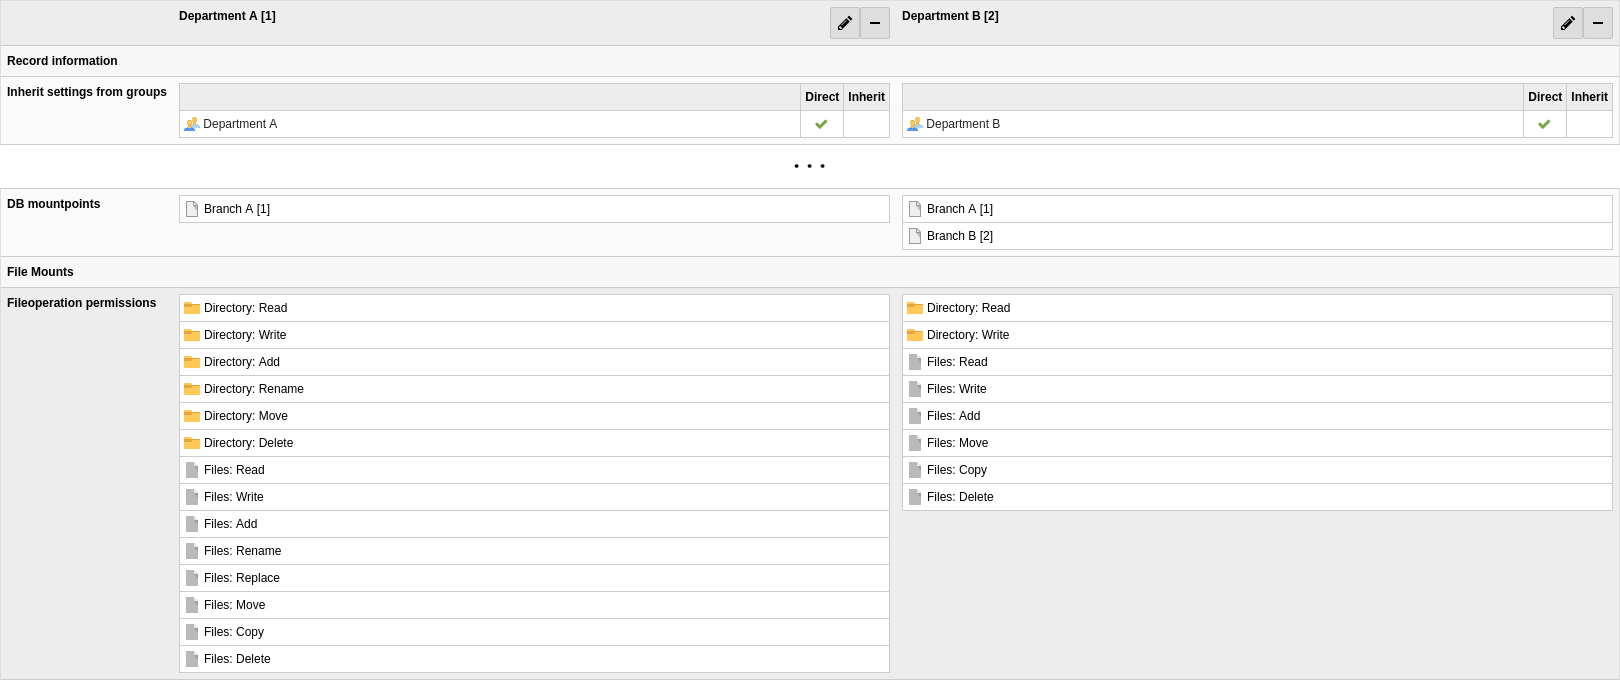
\includegraphics[width=0.9\linewidth]{ChangesForIntegrators/90826-CompareBackendUsergroups.png}
	\end{figure}

\end{frame}

% ------------------------------------------------------------------------------
% Important | 89555 | Workspace-related database records contain the proper Page ID

\begin{frame}[fragile]
	\frametitle{Izmene za integratore}
	\framesubtitle{Workspaces}

	\begin{itemize}
		\item Godinama je jezgro TYPO3 postavljalo \texttt{pid} na vrednost \texttt{-1} za rekorde koji nisu objavljeni.
		\item TYPO3 sada updavlja verzijam rekorda validacijom sledeća tri polja:

			\begin{itemize}
				\item \texttt{t3ver\_wsid} (ID workspace-a u kome je rekord verzionisan)
				\item \texttt{t3ver\_state} (tip verzionisanog rekorda)
				\item \texttt{t3ver\_oid} (objavljena verzija rekorda)
			\end{itemize}

		\item Stoga, \texttt{pid=-1} više nije obavezan.
		\item Upgrade Wizard konvertuje sve \texttt{pid} vrednosti verzionisanih rekorda
			u prave \texttt{pid} vrednosti.
		\item Ova izmena ne utiče na nove instalacije .

	\end{itemize}

\end{frame}

% ------------------------------------------------------------------------------
% Deprecation | 91030 | Runtime-Activated Packages

\begin{frame}[fragile]
	\frametitle{Izmene za integratore}
	\framesubtitle{Proširenja aktivirana tokom vremena izvodjenja}

	\begin{itemize}
		\item Sledeća globalna konfiguracija je označena kao \textbf{zastarela}:\newline
			\smaller
				\texttt{\$GLOBALS['TYPO3\_CONF\_VARS']['EXT']['runtimeActivatedPackages']}
			\normalsize
		\item Korišćenje proširenja aktiviranih tokom vremena izvodjenja značajno usporava TYPO3 instalaciju.
		\item Integratorima se savetuje da preduzmu neophodne korake ukoliko se ova upozorenja pojave u logu zastarelosti:\newline
			\begingroup
				\fontsize{8}{10}
				\texttt{Support for runtime activated packages will be removed in TYPO3 v11.0.}
			\endgroup

	\end{itemize}

\end{frame}

% ------------------------------------------------------------------------------
